\documentclass[a4paper, 12pt]{report}
\usepackage[pdftex]{graphicx}
\usepackage[utf8]{inputenc}
\usepackage{microtype}
\usepackage{amsmath}
\usepackage{url}
\usepackage{dtklogos}
\usepackage{listings}
\usepackage{color}
\usepackage{thesis}
\usepackage[titletoc]{appendix}
\usepackage[tocflat]{tocstyle}
\usetocstyle{standard}

\renewcommand{\UrlFont}{\small\tt}
\makeatletter
\def\footnoterule{\kern-8\p@
\hrule \@height 1pt \@width 6in \kern 7.6\p@}
\renewcommand{\thempfootnote}{\arabic{mpfootnote}}
\makeatother

\lstset{language=C++,
basicstyle=\ttfamily,
keywordstyle=\color{blue}\ttfamily,
stringstyle=\color{red}\ttfamily,
commentstyle=\color{green}\ttfamily,
morecomment=[l][\color{magenta}]{\#}
}

\lstset{language=C++,
keywordstyle=\color{blue},
stringstyle=\color{red},
commentstyle=\color{green},
morecomment=[l][\color{magenta}]{\#}
}

\title{The iCub Cognitive Robotic Experiments}
\author{Semih Onay}
\program{Computer Science}
\supervisor{Assistant Professor Elena Battini Sönmez}

\begin{document}
\pagenumbering{arabic}
\makecstitle
\tableofcontents

\begin{symabbreviations}
  \sym{YARP}{Yet Another Robot Platform}
  \sym{ACE}{The ADAPTIVE Communication Environment} 
  \sym{ODE}{Open Dynamics Library}
  \sym{OpenGL}{Open Graphics Library}
  \sym{SDL}{Simple DirectMedia Layer}
\end{symabbreviations}
\chapter{ABSTRACT}
Intelligent agents with human level of proficiency is the ultimate challenge 
for science and technology. Especially for the artificial intelligence field. 
Desing of such systems now eager to evolve and behave like humans. 
Recent discoveries in this field are focused on training  communication 
skills with perception, classification and action which are modelled from 
humans. They are systems that are capable of recieving environmental 
activities(stimulus) and communication. This paper presents a cognitive 
humanoid robot that combines abilities such as object detection, image 
aqusition, language and movement. Aim is to understand how motor control 
abilities, visio motor abilities and linguistics are designed and developed. 
Study includes robotic simulation applications. Cognitive modules will be 
developed by using application templates and documentation.
\linebreak[2]

\textbf{Keywords :} Cognitive science, Humanoid robots, icub

\chapter{ÖZET}

Günümüzde insansı zekaya ve görünüme sahip robotların tasarımlanması en büyük 
zorluklardan biri olarak karşımıza çıkmaktadır. Geleneksel yapay zeka 
yaklaşımlarının etkisiz kaldığı bu alanda yeni yaklaşımların ortaya çıkması ile 
süregelen bu değişim farklı bir yoldan devam etmektedir. Günümüz yaklaşımları 
daha çok iletişim ve beceri kazanma alanlarında insan modeli üzerinden 
çalışmalar yürütülmektedir. Algıların insanlarda olduğu gibi çevreyi anlamasına 
yardımcı olması ve bunların birer uyartı (stimuli) olarak alması görsel motor 
haraketleri robotlar içinde bir ilham kaynağı olmuştur. Bu çalışmada insana 
benzeyen bilişsel robot üzerinde, görüntü yakalama, dil kavramları, nesne 
ilişkileri ve durumlara göre hareket eylemleri incelenecektir. Amaç olarak 
bilişsel robotik sistemlerin nasıl tasarlandığı, geliştirildiğini ve bu 
sistemlerin nasıl çalıştığını anlamak amacı ile denemeler ve gözlemler 
yapılacaktır.
\chapter{INTRODUCTION}
The iCub is a humanoid robot that developed at \textbf{Istituto Italiano di 
Tecnologia (IIT)} as part of European project RobotCub and later adopted by 
more 
than 20 laboratories arround the world. It has 53 motors that can move the 
head, arms and hands, midriff, and legs.It can see and hear, it has the sense 
of proprioception\footnote{Body configuration and movement using accelerometers 
and gyroscopes}. It’s designed to aid studies of human cognition and artificial 
intelligence. Project members developed computer simulator to experiment new 
techniques.\par 
Computer simulations are getting important in area robotics area. Simulations 
may not provide real complexity of the physical world and 
not reliable as real dynamics. The simulator of iCub is an easy way to test 
new algorithms and methods instead of dealing with complex configuration of 
iCub hardware. The simulator is designed to be accurate as real world 
psychics and dynamics. Development is based on directly from first prototype 
of simulation environment Webots.\footnote{Webots : 
  https://www.cyberbotics.com}It was 
expensive and had limited access to source code which made hard to modify 
source code in order to add some functionalties.Then iCub simulation created. 
Simulation environment uses \linebreak to simulate body 
movement and collision detection algorithms to measure psychical interaction 
with the world. ODE\footnote{Open Dynamics Engine : http://www.ode.org} is 
used in wide range of projects like GAZEBO\footnote{GAZEBO : 
  http://gazebosim.org}ODE is an open source physics engine forauthoring 
  tools, 
computer games,etc. It uses OpenGL\footnote{Open Graphics Library : 
  https://www.opengl.org} renderer and it has some disadvantages due to 
limitation of OpenGL engine computation efficiency on complex structures. 
iCub 
simulation is using OpenGL directly via SDL\footnote{Simple DirectMedia Layer 
: 
  https://www.libsdl.org}which helps to render complex robot movements and 
computationally efficient simulation observations. The aim of this study is to 
experiment and understand how cognitive architecture of robotics designed and 
implemented. 

\chapter{LITERATURE REVIEW}
Development of simulator is described by abstraction of parts to handle 
complex instructions more precisely and efficient. Some other external 
software 
libraries are used to reduce required time to animate given parts of robots 
body from parameters. Abstractions made it easy to implement new 
methods,algorithms into a simulation environment. Understanding of these 
libraries are the key of creating new interfaces and methods to robot in 
virtual world. Action primitives are predefined inside a simulation 
environment to extendcapability of creating new interfaces to virtual 
simulation world and can be changed or taught as different languages which 
helps to extend knowledge about languages.

The great challenges in robotics is to imitate human behaviour. Most of the 
humanoid robots have some perception to recognize their surroundings 
autonomosly. Grasping an object in its environment, is one of the most 
difficult tasks for all kinds of robots. Many parameters must be provided for, 
the objects, surroundings, and the specification of the assignment. Taking 
these parameters into consideration, the ability to receive sensing information 
from the robot is crucial when implementing an efficient robotic grasp. The 
quality of the sensing information 
must also be taken into consideration, as signals may limit precision and can 
potentially be noisy. In recent years, there have been several models 
implemented to perform a grasping behavior.\textbf{\cite{vernon}}
\begin{itemize}
\item Knowledge based grasp action,
\item Geometric grasp action,
\item Sensor driven and learning based grasping.
\begin{figure}[h!]
\centering
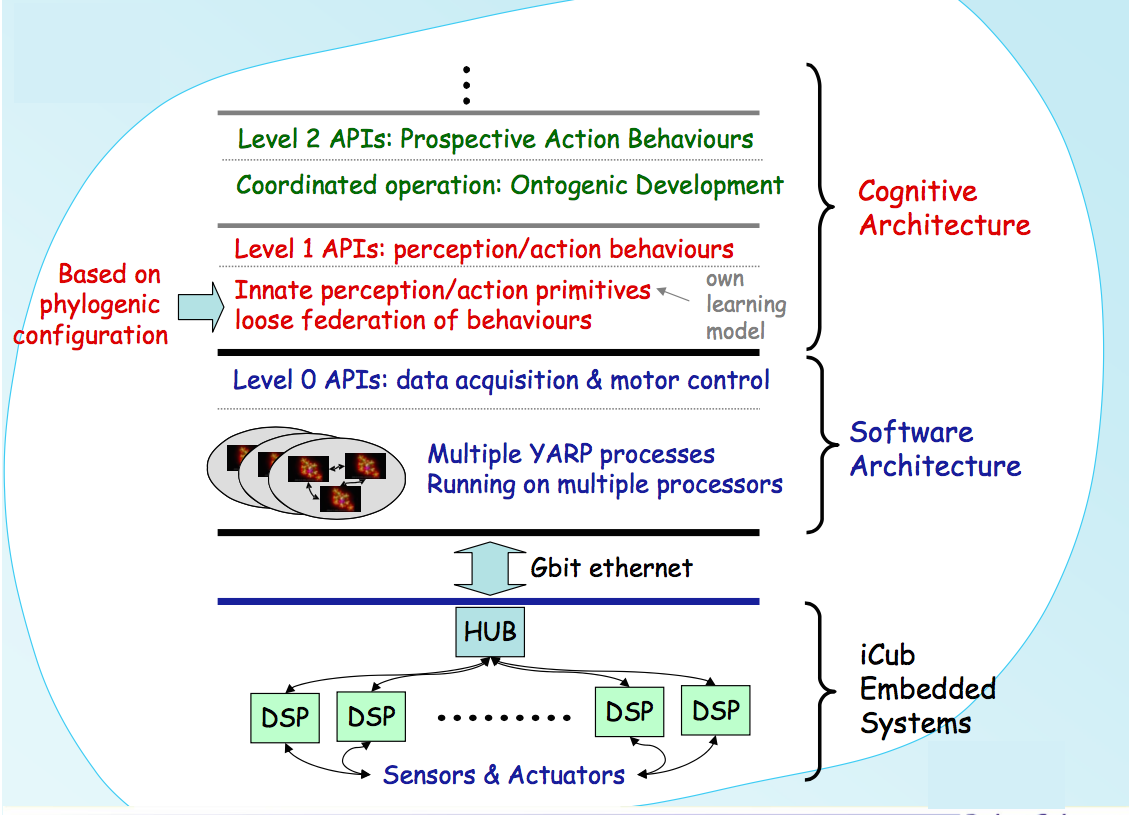
\includegraphics[width=0.7\linewidth]{generalView}
\caption{General View of iCub}
\label{fig:generalView}
\end{figure}
\end{itemize}
\chapter{METHODOLOGY}
\section{The iCub Cognitive Architecture}
The architecture consists of modules and sub modules. Their relations are 
similar to the human mental system. Gaze controling, reaching, and locomotion 
establishes the simple goal oriented actions. Episodic and procedural memories 
are effects a simple version of an internal simulation to provide capabilities 
for prediction and reconstruction, as well as productive model construction 
by experienced affordances from environmental sensors. A simple process of 
homeostatic state is achived by the affective state that provides action 
selection and attention selection. These futures are already implemented in the 
simulation environment.
\begin{figure}[h!]
  \centering
  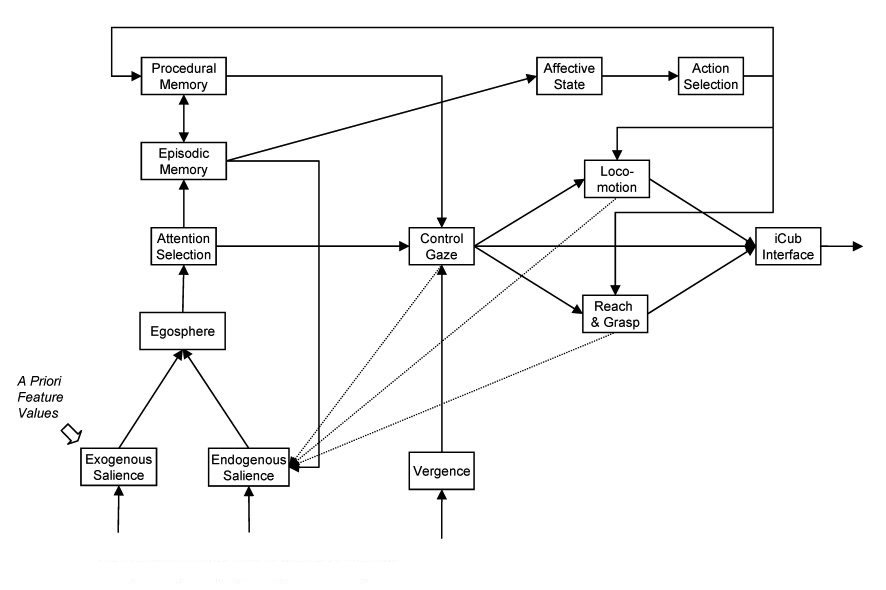
\includegraphics[width=1.0\linewidth]{cognitive_architecture}
  \caption{General View of iCub Cognitive Architecture}
  \label{fig:cognitive_architecture}
 \end{figure}
Indiviual components of the architecture operates synchronously for a series of 
states representing cognitive behaviour that emerges from the interaction of 
separate parallel processes instead of being governed by some state machine as 
it like the most of cognitive architectures. In addition, motivations are 
encapsulated in the affective state of the system. They are designed explicitly 
to address curiosity and experimentation by using explorative motives which are 
triggered by exogenous and endogenous factors, respectively. Distinction 
between the exogenous and endogenous salience is represented by the need to 
include an attention system to consolidate both factors.
\newpage
\section{The Embodiment}
It is developed as an embodied agent by its physical components joints, 
actuators, and a many of sensors that are providing internal stimuli and 
external stimuli information about the body and its 
surroundings.\textbf{\cite{vernon}} 
Actuation is effected through a variety of DC motors and servo motors. Sensory 
data provides joint position, velocity of movements, and torque, streamed video 
images from the head eye cameras, audio from the left and right ear 
microphones. Accessing to the motor control and sensor 
interface is provided through iCubInterface in the cognitive architecture in 
Fig. 5.1 This module is represented as an YARP software module iCubInterface.
That interface turns relevant data into actions.
\section{Software Representation}
Software implementation is shown in Figure 5.2 has been realized as a complete 
software system consist of a YARP and iCub modules. All modules are connected 
internally and communicates through YARP ports and they can be called from a 
application or from command line interface with required paramaters. These 
modules are:
\begin{itemize}
  \item salience
  \item endogenousSalience
  \item egoSphere
  \item attentionSelection
  \item episodicMemory
  \item proceduralMemory
  \item affectiveState
  \item actionSelection
  \item controlGaze2
  \item logPolarTransform
  \item cameraCalib
\end{itemize}
\begin{figure}[h!]
  \centering
  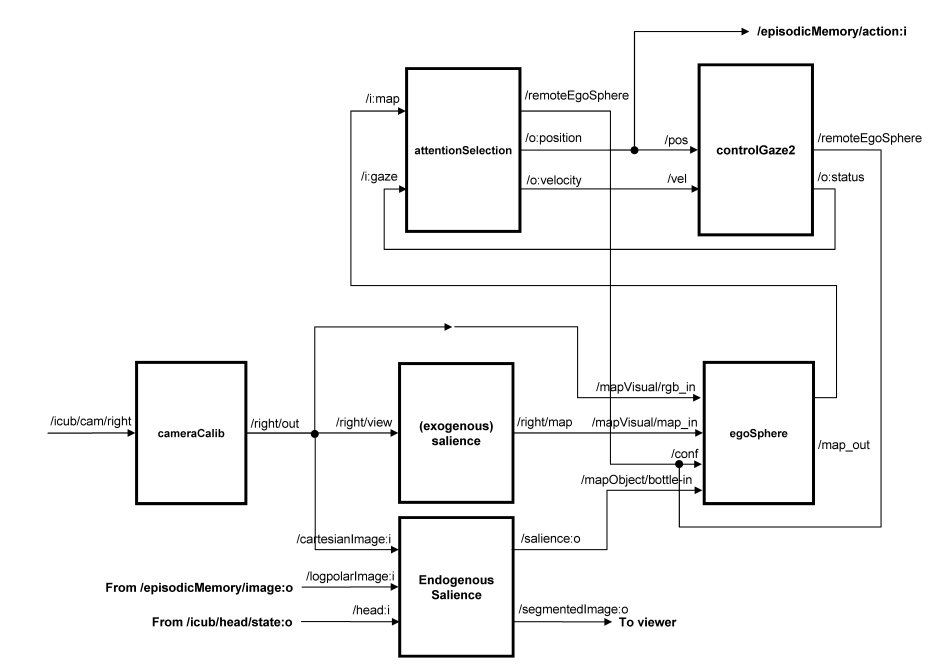
\includegraphics[width=0.8\linewidth]{cognitive_architecture_A}
  \caption{iCub Internal Architecture}
  \label{fig:cognitive_architecture_A}
\end{figure} 
\section{Gaze Control}
The Gaze Control component provides coordinated control of the head and eyes of 
the iCub. Rather than by specifying the raw joint values for the head and eyes, 
the gaze direction of the robot is specified by gaze direction (azimuth and 
elevation angles) and vergence of the two eyes. In addition, the motion of the 
eyes and head when moving to a given gaze position are controlled to provide a 
motion profile that is similar to humans, with the gaze direction of the eyes 
moving quickly and the head moving more slowly but subsequently catching up so 
that the eyes gaze is reaching an equilibrium position that is relatively 
centred with respect to the head  and with the head oriented in the specified 
gaze direction.
\newpage The gaze direction can be specified using any of four different types 
of 
coordinates:
\begin{itemize}
  \item absolute azimuth and elevation  in degrees;
  \item azimuth and elevation angles relative to the current gaze direction;
  \item normalized image coordinates (in the range zero to one) of the position 
  at which the iCub should look;
  \item the image pixel coordinates of the position at which the iCub should 
  look.  Head gaze and vergence are controlled simultaneously.
\end{itemize}
There are two modes of head gaze control: saccadic motion and smooth pursuit
motion. Saccades are controlled in two phases. In the first fast phase, the 
eyes are driven quickly to the destination gaze direction by controlling the 
common eye ver- sion and tilt degrees of freedom. In the second slow phase, the 
neck moves toward the final gaze direction with a slower velocity profile and 
the eyes counter rotate to keep the image stable. A new saccade is accepted 
only when the previous one has finished. This is the typical operation in 
humans where saccades are used to change the object of interest. Smooth 
pursuit only operates in the slow phase, but it accepts a continuous stream 
of commands.\textbf{\cite{cangelosi-action}}It is meant to emulate the human 
behaviour 
when 
tracking an 
object. A single set of motor controller gains are used for both the saccade 
and smooth pursuit modes. These gains specify the speed of the motion and 
therefore the amount of motion undergone by the eyes and by the neck. The 
higher the gain, the more the eye motion will lead the neck motion and, 
therefore, the more the eyes have to counter rotate as the neck approaches the 
gaze direction. Vergence operates continuously in a single phase and there is 
an independent gain for the vergence controller.
\section{Reach and Grasp}
The Reach and Grasp includes a robust task space reaching controller 
for learning internal generic inverse kinematic models and human-like 
trajectory generation. This controller takes into account various constraints 
such as joint limits, obstacles, redundancy and singularities. It also includes 
a module for grasping based on reaching and orienting behaviours. This allows 
the coordination of looking (for a potential target), reaching for it (placing 
the hand close to the target) and attempting a grasping motion (or another 
basic action).
At present, the reaching controller takes as input the Cartesian position and 
orientation of an object to be grasped, based on a visual recognition 
process. The arm and torso configuration to achieve the desired pose (hand 
position and orientation) is determined by a non linear optimizer 
which takes into account all the various constraints, one of which is to keep 
the torso as close as possible to vertical while reaching. Subsequently, 
human like straight hand and arm trajectories are then generated 
independently using a biologically inspired controller.\textbf{\cite{lorenzo}} 
This 
controller 
exploits a multi referential system whereby two minimum velocity
vectors are generated, one in joint space and one in task space. A 
coherence constraint is imposed which modulates the relative influence of the 
joint and task space trajectories. The advantage of such a redundant 
representation of the movement is that a quasi straight line trajectory 
profile which is similar to human like motion can be generated for the hand in 
the task space while at the same time retaining convergence and robustness 
against singularities.
\section{Action}
Guideline 10 states that movements should be organized as actions. Since 
actions are planned, goal oriented, acts they are triggered by system 
motivation and they are guided by prospection. The action is defined, not by a 
servo motor set point specifying an effector movement, but by the goal of the 
action, an action whose outcome must be achieved adaptively by constituent 
movements. This guideline is implemented in the iCub cognitive architecture by 
the procedural and episodic memories and by use of visual servoing in reaching 
and locomotion\textbf{\cite{xavier}}. Specifically, the procedural memory 
represents 
actions as gaze 
saccades together with an optional reaching, hand pushing, grasping, or 
locomotion movement. These actions are associated with expected outcomes 
defined by the expected outcome in the episodic memory. Thus, the procedural 
and episodic memory provide a feed forward goal state for the action while the 
visual servoing, whereby the effector is adaptively controlled to align it with 
a fixation point while re centering the gaze after the execution of eye 
movement, achieves the required motion through feedback control of the arm and 
hand.
\newpage
\section{Action Selection}
The purpose of the Action Selection component is to effect the development of 
the iCub and specifically to increase its predictive capability. In the current 
version of the iCub cognitive architecture, this means the selection of the 
iCub’s mode of exploration. At present, only two basic motives drive this iCub 
development, curiousity and experimentation, both of them exploratory. The 
third main motive, social interaction, has not yet been 
addressed.\textbf{\cite{vernon}} 
Consequently, the present implementation of action selection is based on a very 
trivial function of the levels of curiousity and experimentation produced by 
the Affective State component. Specifically, the learning mode is selected if 
the curiosity level is higher than the experimentation level; otherwise the 
prediction mode is selected.
\section{The YARP}
It is a set of open source libraries that supports modularity by 
using abstraction method in softwares to handle common difficulties in 
robotics area which are know as modularity algorithms, hardware interfaces and 
OS platforms.To deal with OS spesific builds,requires to use cross-platform 
build tools such as CMake\footnote{CMake : http://www.cmake.org} and 
ACE\footnote{The ADAPTIVE Communication Environment :
  http://www.cs.wustl.edu/~schmidt/ACE.html}. YARP is providing platform 
independence. First abstraction can be described as a protocols. Main YARP 
protocol manages interprocess communications in operating systems. It can 
deliver process messages of any size across the network by using different 
protocols.
\begin{figure}[h!]
  \centering
  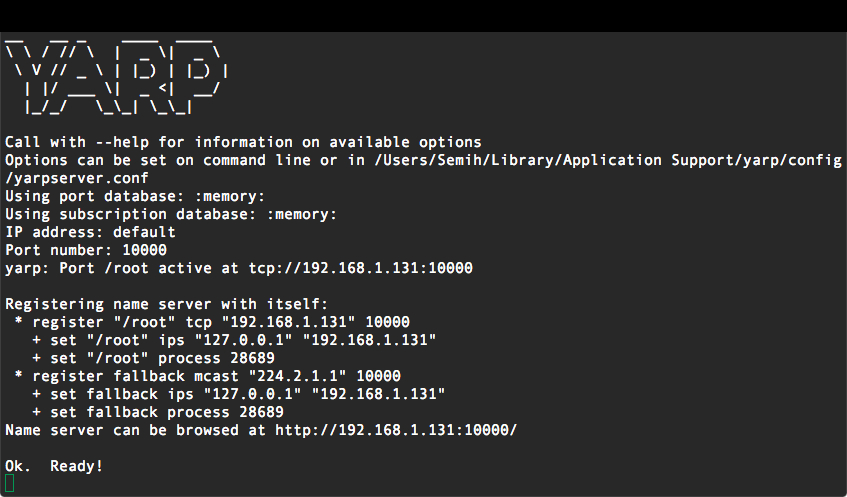
\includegraphics[width=1.0\linewidth]{yarp}
  \caption{YARP Command Line Interface}
  \label{fig:yarp}
\end{figure}
Second abstraction is about hardware communications.The method is to define 
interface for class of devices to fold native coded APIs.Changes in hardwares 
requires changes in API\footnote{API : Application Programming Interface} calls 
via linking suitable libraries to encapsulate 
hardware dependency problems. These abstractions combined to use remote 
device drives where that can be accessed across the network like a parallel 
processing.
The purpose of YARP ports are to move data from threads to threads over the 
processes.Flow of the data can be configured and observed from command-line 
at real time. Port can receive or send data from any other port.Connections 
between ports can be modified easily with using different protocols such as 
TCP\footnote{TCP : Transmission Control Protocol} and UDP\footnote{UDP : User 
Datagram Protocol}.The choice depends on quality of message transmission or 
response 
time. Using TCP is for reliability and UDP is for speed with effect on 
unreliable transmissions. As it seen in Figure 4.3 it registers a name server 
over localhost and assigns root node to branching iCub components. YARP 
contains abstraction of many classes which are called as “Bottle”. That helps 
to develop more sophisticated applications by abstraction.
\newpage
\section{iCub Simulation Environment}
The computer simulation model of the iCub allows to create realistic scenarios 
in where robot can interact with a virtual world and physical limitations, 
interactions that occur between the virtual world is simulated using open 
source library ODE to provide accurate simulation of body dynamics.
Simulation surroundings can be manipulated by a single configuration file which 
contains ; textures, objects, default arm positions, video configurations and 
calibration settings. In order to place some objects in the environment, it 
needs to be spawned by using the command line interface. Environment supports 
direct frame streaming through yarpview application.
\begin{figure}[h!]
\centering
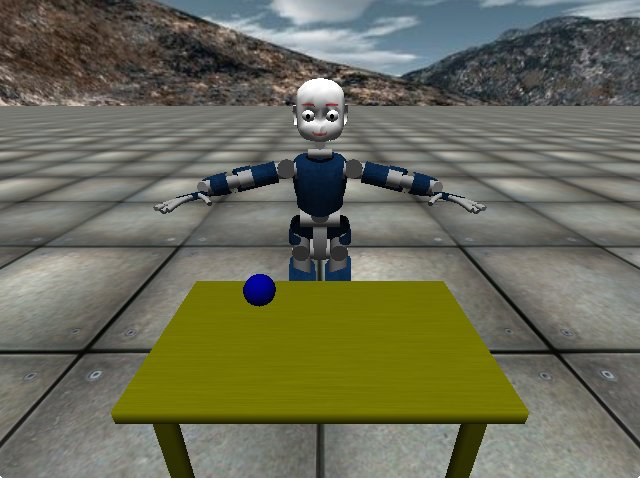
\includegraphics[width=0.5\linewidth]{sim}
\caption{iCub Simulation Environment}
\label{fig:icub}
\end{figure}
\chapter{CONCULUSIONS}
\section{Speech Synthesis}
Speech module has ability to speak given text inputs only in English language. 
A new Module developed from application template with open source text to 
speech library. iCub now can speak Turkish language. Module can be extended to 
synthesis of another languages. eSpeak wrapper can provide various of language 
sound database. Speech Recognition module exists but it needs some Windows 
system libraries.
\section{Speech Recognition}
Implementation of Turkish Language recognition was not possible due to lack of 
grammar files, tokens and lack of NLP resources on Turkish language. Sample 
module tested with English commands and it can give Turkish feedback.
\section{Object Grasping}
Module tested with example data sets. It can grasp an object from table. It 
requires that other modules support. Required modules must be running before 
the grasping module. It needs to be trained from a neural network file.
\section{Image Capture}
An application developed from templates to capture actual action sequences from 
head camera. Images can be streamed as a video.
\section{Sound I/O}
Small module developed to send sound commands from computer microphone. Module 
documentation was not enough descriptive to create new audio ports for speech 
recognition. Some applications were not complied at all. iCub can recive and 
understand speech commands.
\section{Action Primitives}
Application created from the template to understand how robot recognizes and 
performs actions.
\section{Full Body Movement}
All parts of the iCub experimented by developed application. Program takes 
paramaters from iCub root directory which are .ini files.
\section{Arms Control}
Left and right arms experimented by developed application. It may contain some 
bugs due to lack of official documentation. Program can take parameters from 
simulation environment.
\par 
Implementations are avaible at 
\textbf{\url{semyonic.github.io/iCubExperiments/}}
\chapter*{}
\centering Page is intennionaly left blank
\appendix
\chapter{Sample Code Snippets}
\section{Turkish Synthesis Module}
\begin{lstlisting}
class iSpeak : protected BufferedPort<Bottle>,
public    RateThread
{
string name;
string package;
string package_options;
deque<Bottle> buffer;
Mutex mutex;
bool speaking;
MouthHandler mouth;
// gets text sequence
void speak(const string &phrase)
{
string command("echo \"");
command+=phrase;
command+="\" | ";
command+=package;
command+=" ";
// Check for speech synthesis library
if (package=="espeak")
command+="-v turkish --stdin";

// Get text input from CLI
command+=package_options;
//int ret=system(command.c_str());
}
void run()
{
string phrase;
double time;
bool onlyMouth=false;
int rate=(int)mouth.getRate();
bool resetRate=false;
double duration=-1.0;

mutex.lock();
// protecting also the access of size() function
if (buffer.size()>0)    
{
// allocate space from yarp Bottle
Bottle request=buffer.front();
buffer.pop_front();

if (request.size()>0){
  if (request.get(0).isString()){
      phrase=request.get(0).asString().c_str();
      speaking=true;
  }
else if (request.get(0).isDouble() || request.get(0).isInt())
  {
time=request.get(0).asDouble();
speaking=true;
onlyMouth=true;
}
}
\end{lstlisting}
\newpage
\section{Object Mover Module}
\begin{lstlisting}
public:objectMoverThread(ResourceFinder &_rf) : rf(_rf) {
virtual bool loadParams() {
name = rf.check("name",Value("objectMover")).asString().c_str();
neckTT = rf.check("necktt",Value(2.0)).asDouble();
eyeTT = rf.check("eyett",Value(1.2)).asDouble();
trajTime = rf.check("trajtime",Value(4.0),"Solver trajectory 
time").asDouble();
maxPitch = rf.check("maxpitch",Value(30.0),"Torso max pitch").asDouble();

//get which arm to use. default to left if they didnt pass in left or right
armname = rf.check("arm", Value("left"),"arm name").asString().c_str();
if (armname == "right") {
armInUse = true;
}
else {
armInUse = false;
}
//get robot name to use (icubSim is for simulation)
robotname = rf.check("robot", Value("icubSim"),"robot name").asString().c_str();
}
\end{lstlisting}
\chapter{Screenshots}
\begin{figure}[h!]
  \centering
  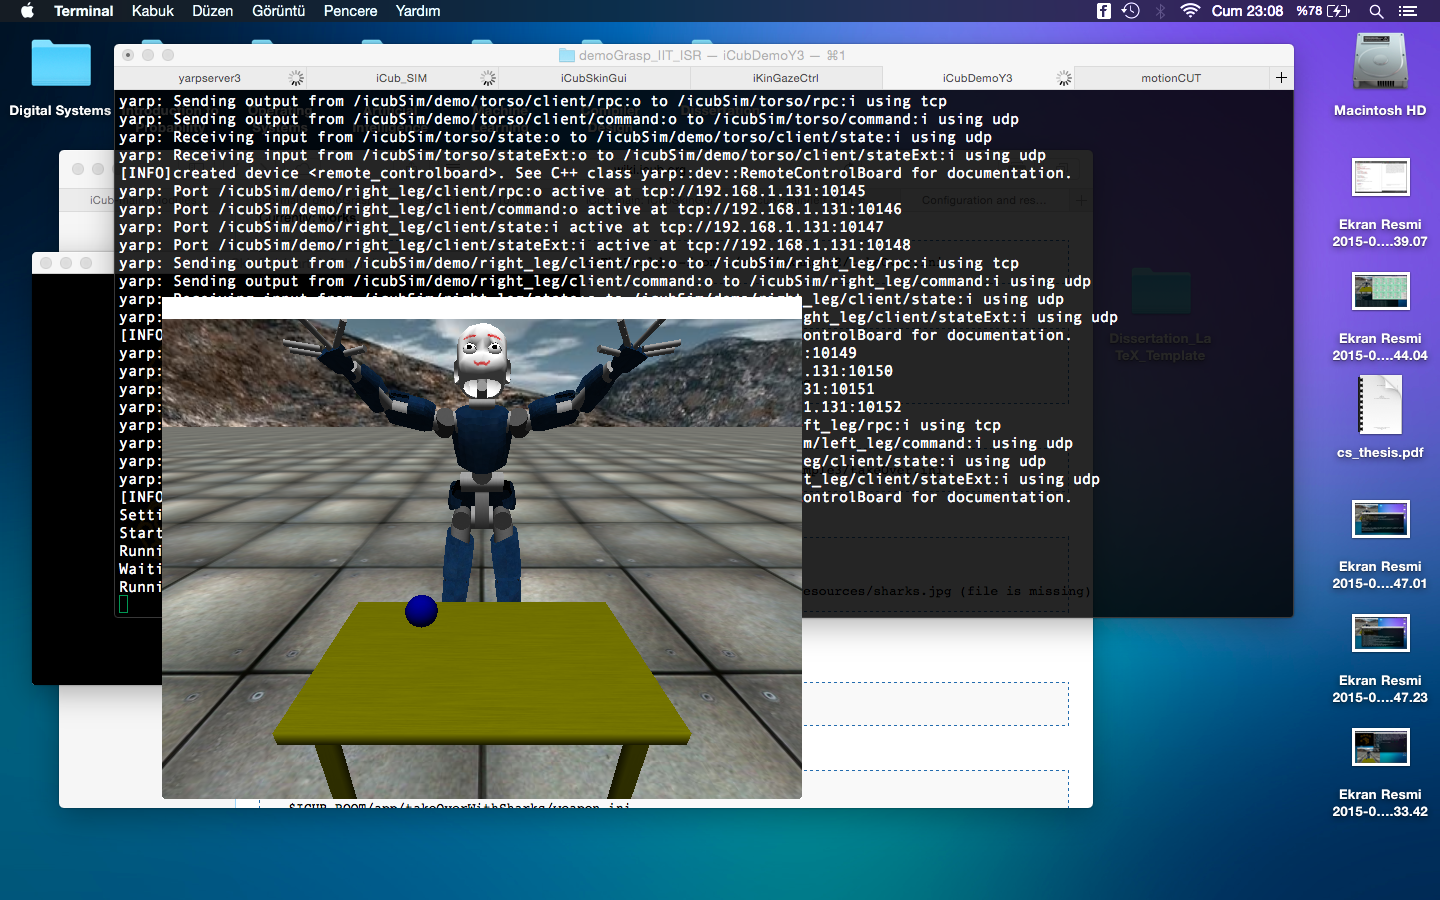
\includegraphics[width=1.0\linewidth]{fullBody}
  \caption{Full Body Movement}
  \label{fig:fullBody}
\end{figure}
\begin{figure}[h!]
\centering
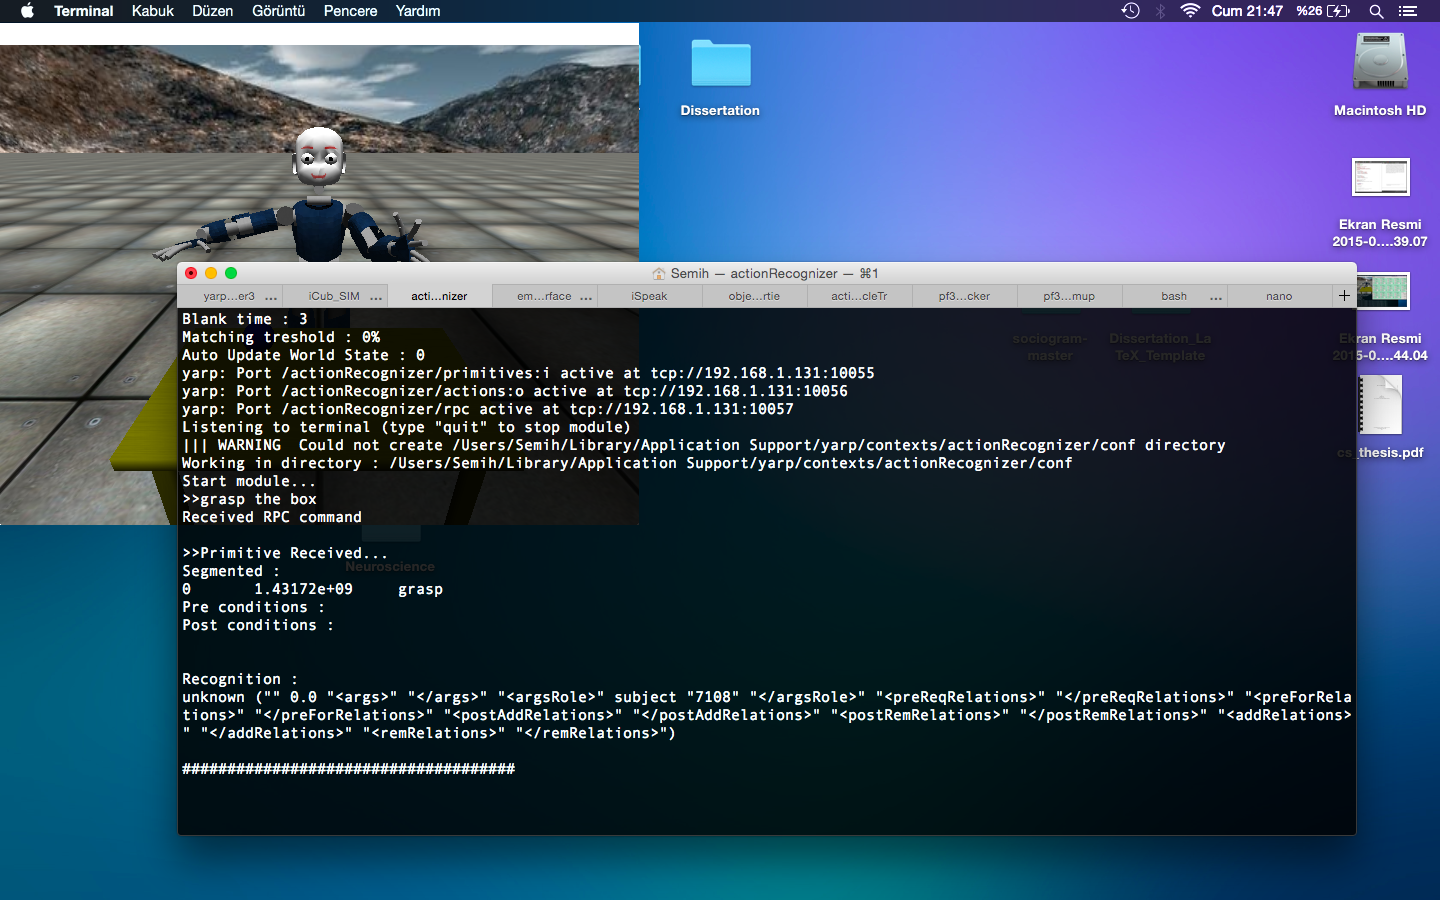
\includegraphics[width=1.0\linewidth]{actionRecognizer}
\caption{Action Recognizer}
\label{fig:actionRecognizer}
\end{figure}
\begin{figure}[h!]
\centering
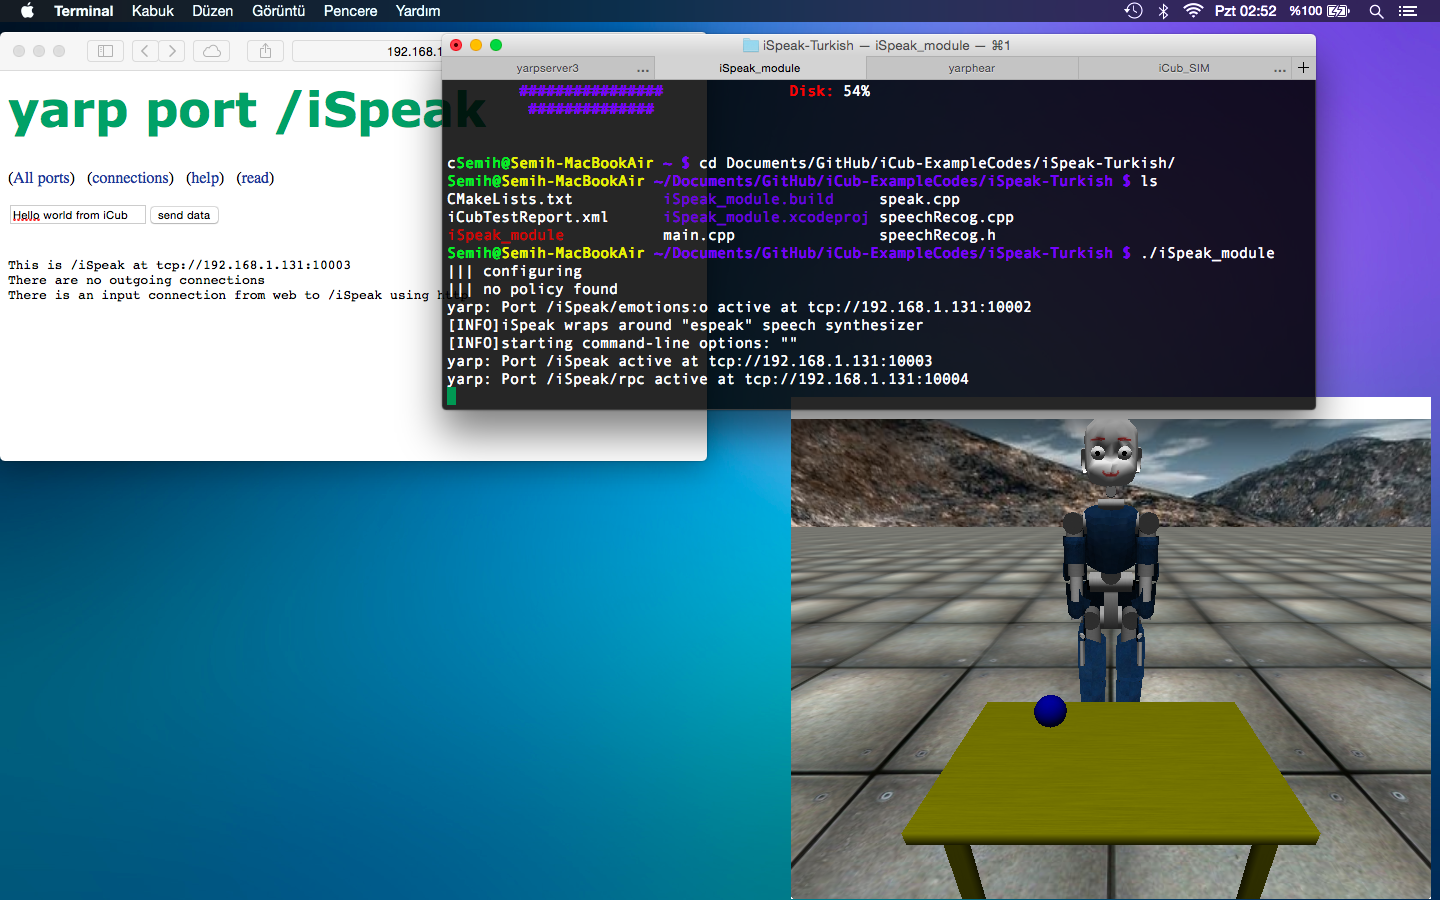
\includegraphics[width=1.0\linewidth]{iSpeak}
\caption{iSpeak Module}
\label{fig:iSpeak}
\end{figure}
\begin{figure}[h!]
\centering
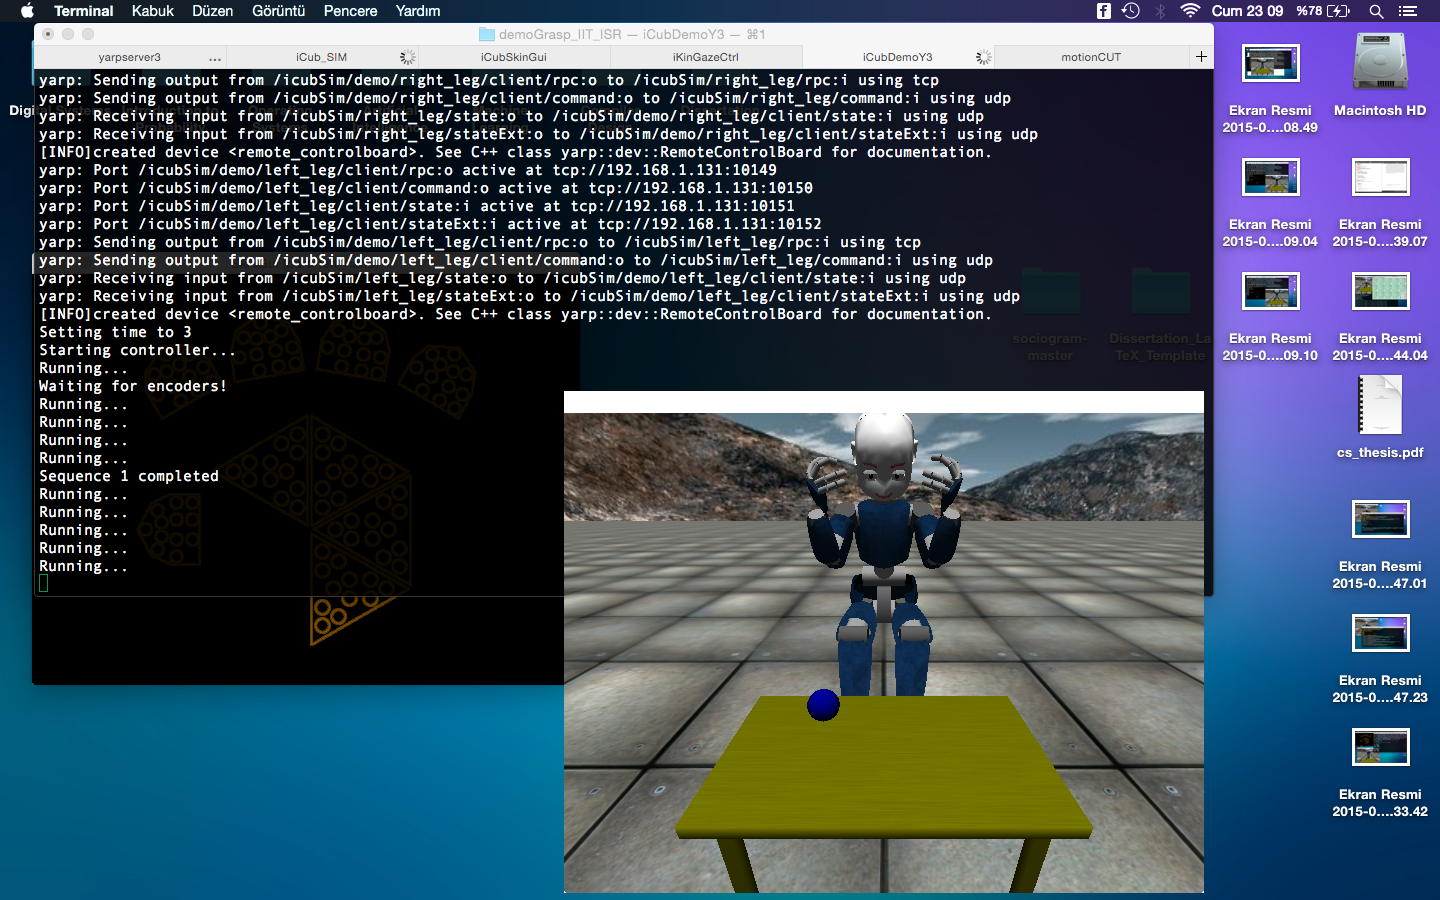
\includegraphics[width=1.0\linewidth]{neural}
\caption{iCub Sample Body Postures}
\label{fig:neural}
\end{figure}
\begin{thebibliography}{9}
  
  \bibitem{cangelosi-action}Tikhanoff, V.; Cangelosi, A.; Metta, G., 
  "Integration of Speech and Action in Humanoid Robots: iCub Simulation 
  Experiments," Autonomous Mental Development, IEEE Transactions on , vol.3,
  
  \bibitem{vernon} A Roadmap for Cognitive Development in Humanoid Robots, 
  David Vernon,Claes von Hofsten,Luciano Fadiga, 2010
  
  \bibitem{lorenzo} The iCub humanoid robot: an open platform for research in 
  embodied cognition, Giorgio Metta Giulio Sandini, David Vernon, Lorenzo Natale
  Francesco Nori, 2008
  
  \bibitem{simulator}The iCub Humanoid Robot Simulator,V.Tikhanoff, 
  P.Fitzpatrick, F.Nori, L Na- tale, G.Metta and A.Cangelosi, 2010
  
  \bibitem{xavier}Real-Time Parallel Processing of 
  Grammatical Structure in the Fronto-Striatal System: A Recurrent Network 
  Simulation Study Using Reservoir Computing , Hinaut X, Dominey PF , 2013
  
  \bibitem{icub} The iCub-main: iCub Software Repository Documentation, 
  \url{http://wiki.icub.org/iCub_documentation/} Last Acess : 01.June.2015 
  
  \bibitem{install} Getting the iCub software, 
  \url{http://eris.liralab.it/wiki/Getting_the_iCub_software} Last Access : 
  01.June.2015
  
  \bibitem{tutorials} https://github.com/robotology/icub-tutorials 
  \url{https://github.com/robotology/icub-tutorials} Last Access : 01.June.2015
  
  
\end{thebibliography}
\end{document}